\documentclass[11pt, oneside]{article}   	% use "amsart" instead of "article" for AMSLaTeX format
\usepackage{geometry}                		% See geometry.pdf to learn the layout options. There are lots.
\geometry{letterpaper}                   		% ... or a4paper or a5paper or ...
%\geometry{landscape}                		% Activate for rotated page geometry
%\usepackage[parfill]{parskip}    		% Activate to begin paragraphs with an empty line rather than an indent
\usepackage{graphicx}				% Use pdf, png, jpg, or eps§ with pdflatex; use eps in DVI mode
								% TeX will automatically convert eps --> pdf in pdflatex
\usepackage{amssymb}
\usepackage{hyperref}

\usepackage[scaled]{helvet}
\usepackage[T1]{fontenc}
\renewcommand\familydefault{\sfdefault}

\usepackage{parskip}

\title{Linear differential equations}
\author{Albert Xu}

\begin{document}
\maketitle

I'm developing an application to \href{https://github.com/alberttxu/diffeqvisualizer}{visualize differential equations}.
The purpose of this app is to help students understand what a differential equation means,
since many college courses don't provide much intuition.
This document covers the mathematics used in the app's demo examples.

\section{Intro}

A differential equation describes a function in terms of its derivatives.
For example, the linear differential equation
\begin{equation}
\dot{x} = Ax
\end{equation}
says that a function $x(t)$ must equal its derivative $\dot{x}(t) = \frac{dx}{dt}$ when multiplied by $A$.
The word linear means $\dot{x}$ is expressed in terms of multiplications and additions of $x$.
Basically, there are no $x^2$ or $\sqrt{x}$ terms, additional constant terms, etc.
More generally, a differential equation is defined as $\dot{x} = f(x)$,
but for now we will analyze the linear case.

Important notes:
\begin{itemize}
  \item There are many possible solutions for a differential equation (DE).
  In equation (1), $x$ refers to any solution, not necessarily a specific one.
  \item For most complicated DEs there is no closed-form expression that can describe all possible solutions.
  \item For a particular (i.e. specific) solution $x(t)$, it is useful to think of $x$ not as a function, but as some quantity at time $t$ in a simulation.
    \subitem Example: $x$ represents the location of an object, and $\dot{x}$ represents its velocity.
  \item For a particular solution $x(t)$, the set of its past values is sometimes called a trajectory.
  \item The study of a particular solution with a starting value $x_\mathrm{initial}$ at $t = 0$ is called an initial value problem.
\end{itemize}


\section{1D case}

We want to solve equation (1),
$$\dot{x} = Ax,$$
where $A$, $x$, and $\dot{x}$ are numbers.
Let's use a simple example: $x$ is the location of a particle on a number line and $\dot{x}$ is its velocity.

If $A = 0$ then $\dot{x} = 0$, i.e. velocity is zero for all $x$.
For any initial value of $x$, its trajectory never moves.

If $A > 0$ then trajectories will move away from the origin.
Since $\dot{x}$ is proportional to $x$,
if $x > 0$ the trajectory will move further to the right, and if $x < 0$ it will move further to the left.

If $A < 0$ then trajectories will shrink towards the origin using similar logic.

All 3 cases can be described using the general-form solution,
\begin{equation}
x(t) = ce^{tA} .
\end{equation}
However, for a specific particle, its solution is
\begin{equation}
x(t) = x_\mathrm{initial} e^{tA}
\end{equation}
since $x_\mathrm{initial}$ uniquely determines $c$.
\begin{itemize}
  \item Fun fact: this is the same formula used in \href{https://en.wikipedia.org/wiki/Compound_interest#Continuous_compounding}{compound interest}
\end{itemize}


\section{2D case}

This is much more interesting since there are numerous ways a 2D point can move relative to the origin.
I believe it is very hard to understand the dynamics in this case without a graphical application.
And so I encourage the reader to play around with the elements of $A$ to see how it affects the motion of trajectories.
In the rest of this section I won't go into troublesome formulas and derivations like in most college courses,
and instead only mention basic definitions and notation required to understand this section.
Higher dimensional linear DEs are also known as linear dynamical systems.
An excellent course on this topic is taught at Stanford: \url{https://see.stanford.edu/Course/EE263}.
And for those who want a quick infographic,
\url{https://en.wikipedia.org/wiki/Stability_theory} has content that supplements the basics covered here,
although in my opinion the language is a bit dense.

In 2 dimensions, $x$ and $\dot{x}$ are vectors with 2 components (a.k.a elements, entries), and $A$ is a $2\times 2$ matrix.
I won't use fancy LaTeX to emphasize that $A$, $x$, and $\dot{x}$ are not scalars.
Equation (1),
$$ \dot{x} = Ax ,$$
still has the same meaning as before.
We can imagine that $x$ represents a particle's position in a 2D plane,
and $\dot{x}$ represents its direction of travel (velocity).
$A$ is a map from position to velocity: for a particle at position $x$, its velocity must equal $Ax$ regardless of time $t$.

The components of $x$ describe its location along individual axes.
For example, $x_1$ is the particle's location in the horizontal direction,
and $x_2$ is its location in the vertical direction.
Likewise $\dot{x}_1$ and $\dot{x}_2$ represent individual velocity components.

If you play around with the entries of $A$ you will see several kinds of behavior:
rotation;
scaling;
moving away from or towards the origin;
asymptotically approaching seemingly arbitrary axes;
and more.
Here is a screenshot I've taken of the Trajectories demo below.

\graphicspath{ {./assets/} }
\begin{figure}[h]
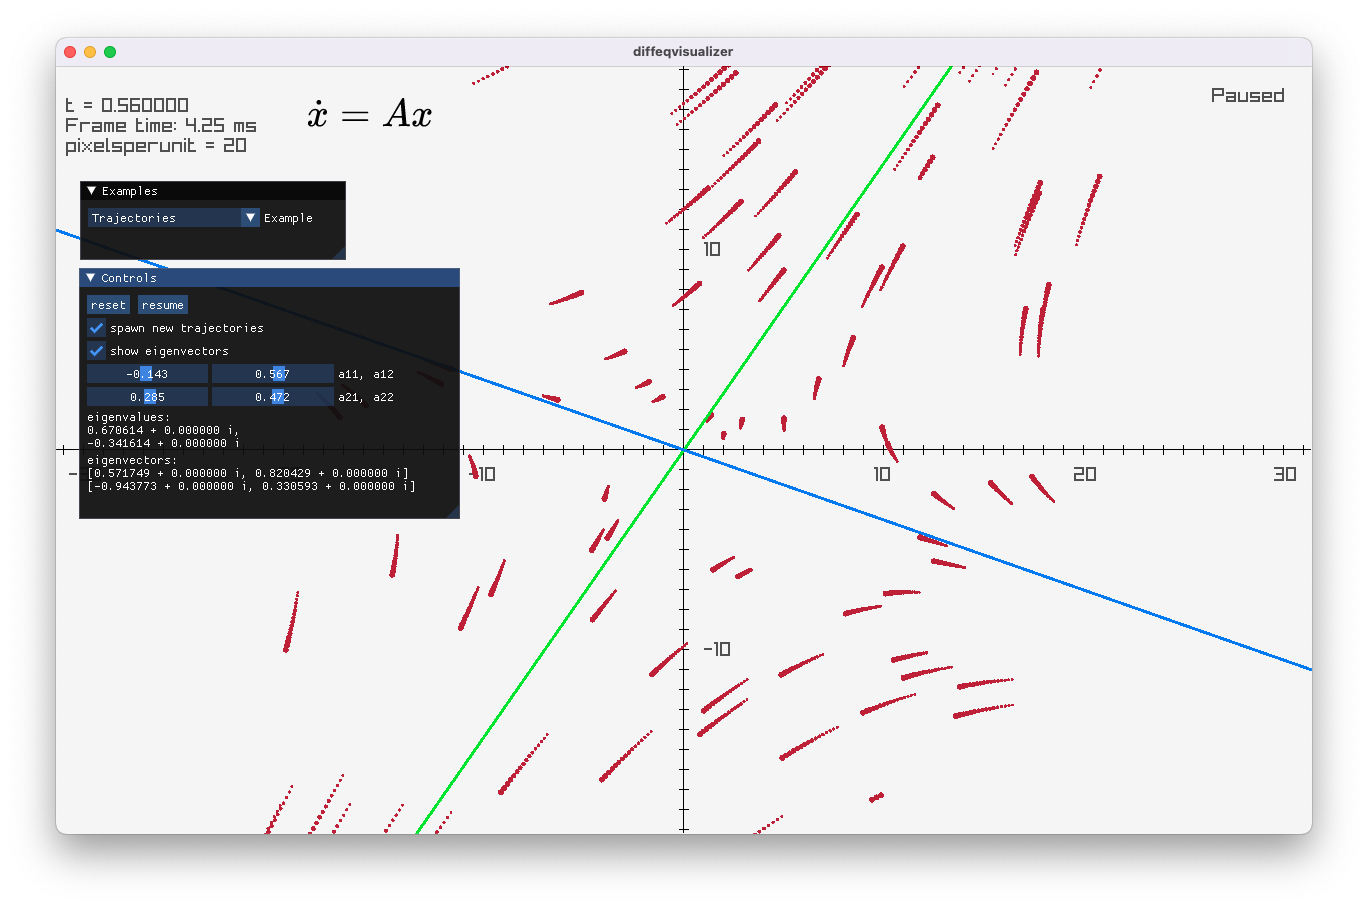
\includegraphics[scale=0.31]{screenshot_trajectories}
\caption{trajectory dynamics of $\dot{x} = Ax$, a.k.a phase space}
\end{figure}

Each red comet is a trajectory.
The tail of each trajectory is drawn by creating cirlces for its most recent values.
You may notice that the trajectories seem to move towards the origin when they are near the blue line,
and are repelled away from the origin near the green line.
This is not a coincidence and it has to do with the eigenvectors of $A$.

\subsection*{Special solution - eigenvector}

An eigenvector of a square matrix, $A$ for example, is a vector $v$ that satisfies the condition
\begin{equation}
Av = \lambda v
\end{equation}
for some $\lambda$.
In the context of our linear DE, $\dot{x} = Ax$, if a trajectory $v$ is an eigenvector of $A$ then
\begin{equation}
\dot{v} = Av = \lambda v
\end{equation}
which is actually the 1D case in each component,
i.e. $\dot{v}_\mathrm{horiz} = \lambda v_\mathrm{horiz}$, $\dot{v}_\mathrm{vert} = \lambda v_\mathrm{vert}$.
Visually this means that $v$ moves either directly towards or away from the origin.
And therefore it may grow or shrink, but cannot rotate - its angle never changes.
Just like in the 1D case, $\lambda < 0$ leads to shrinking, and $\lambda > 0$ leads to growth.
$\lambda$ is called the eigenvalue associated with the eigenvector $v$.

Important notes:
\begin{itemize}
\item Any scaled version of $v$ is also an eigenvector of $A$.
Therefore grammatically it is more correct to say $v$ is \textit{an} (instead of \textit{the}) eigenvector associated with $\lambda$.
The line spanned by $v$ is sometimes called the "eigenspace" associated with $\lambda$, but this terminology is not universally standard.
\item For an $n\times n$ matrix, there are $n$ eigenvector-eigenvalue pairs. However, the eigenvalues are not always distinct.
\item Conventional notation in many fields denotes eigenvectors as $v_i$ using subscripts.
For example: "\textit{Let $ v_1,\cdots,v_n $ be eigenvectors of $A$ with eigenvalues $ \lambda_1,\cdots,\lambda_n $}."
Sometimes this may be confusing since subscripts are also commonly used to refer to scalar elements of vectors.
Be mindful of literary context.
\end{itemize}

\subsection*{General solution}

What if a trajectory $x$ is not an eigenvector of $A$?
The key insight is that we can break $x$ into pieces which \textit{are} eigenvectors.
That is to say, we can find some scaled eigenvectors $v_1$ and $v_2$ of $A$ that satisfy
\begin{equation}
x = v_1 + v_2
\end{equation}
and now it becomes clear how to analyze the trajectory's behavior.
Again, in the context of our linear DE, $\dot{x} = Ax$, we plug in $x$ and get
\begin{equation}
\dot{x} = Ax
= A(v_1 + v_2)
= A v_1 + A v_2
= \lambda_1 v_1 + \lambda_2 v_2
\end{equation}
However, we already know that
$$ \dot{v}_1 = A v_1 = \lambda_1 v_1 $$
$$ \dot{v}_2 = A v_2 = \lambda_2 v_2 $$
with solutions
$$ v_1(t) = v_{1,\mathrm{initial}} e^{t\lambda_1} $$
$$ v_2(t) = v_{2,\mathrm{initial}} e^{t\lambda_2} $$

Let's pause for a second and think about what this implies.
It means that we can independently compute the trajectories for each eigenvector and add them to get the solution for $x$.
Hopefully now it is clear what is happening in Figure 1.
The eigenvectors of $A$ lie on the blue and green lines.
Each trajectory has components in the blue and green directions.
Eigenvectors on the blue line have a negative eigenvalue, and eigenvectors on the green line have a positive eigenvalue.
So over time, the blue component of $x$ shrinks and the green component of $x$ grows.

You might wonder if we can reuse the formula from the 1D solution (equation 3).
\begin{equation}
x(t) = e^{tA} x_\mathrm{initial}
\end{equation}
Due to syntactial reasons we have to swap the order of symbols on the right.
$x(t)$ and $x_\mathrm{initial}$ are vectors, so the term $e^{tA}$ must either be a scalar or a $2\times 2$ matrix.
Spoiler: it's the latter, and the formula is indeed valid in 2 dimensions,
but we need to extend the definition of the exponential function for a square matrix $A$.
This is called the matrix exponential, but how exactly is it defined?
And how does this method compare to the one we just analyzed?
Gilbert Strang at MIT gives some good answers in this \href{https://youtu.be/LwSk9M5lJx4}{youtube video},
so I won't regurgitate them here.
But I will emphasize what the matrix exponential actually does: it \textbf{acts as a time travel operator}.
Given an initial condition $x_\mathrm{initial} = x(0)$, we can compute a trajectory's future value $x(t)$ for any $t$ (equation 8).
Furthermore, given a trajectory's current value $x_\mathrm{current} = x(t)$, we can compute its past value $dt$ seconds \textit{ago}:
\begin{equation}
x(t-dt) = e^{-dtA} x_\mathrm{current}
\end{equation}

See also:
\begin{itemize}
\item 3Blue1Brown has an entire \href{https://youtu.be/O85OWBJ2ayo}{video} dedicated to the matrix exponential.
\item \href{https://www.youtube.com/watch?v=5ePa2UOkEV0&list=PL06960BA52D0DB32B}{Lecture 11} in Professor Boyd's EE263 class
(an essential class for engineering students)
\end{itemize}

\end{document}